\chapter{Réalisation d'une politique de cache de données}
\label{app:cache}
	L'utilisation d'un \gls{cache} permet de stocker des informations et de les conserver jusqu'au moment où l'on souhaite y accéder.

	Dans notre heuristique d'insertion au plus tôt, nous sommes contraints de déterminer après chaque interception quel est le mobile suivant qui pourra être intercepté au plus tôt. Une interception concerne uniquement un mobile et un intercepteur. Ainsi dans un problème à $n$ mobiles et $m$ intercepteurs, à la première interception, $n-1$ mobiles et $m-1$ intercepteurs ne seront pas concernés, soit $n \times m -n -m +1$ dates d'interception potentielles qui resteront les mêmes au calcul de la seconde interception.

	Le calcul des dates d'interception fait appel à plusieurs fonctions trigonométriques et demande donc un temps plus important que pour effectuer des calculs élémentaires. Il est par conséquent impératif de faire le maximum pour réduire le nombre d'appels à ce calcul. Sachant que l'on travaille avec $n$ mobiles et $m$ intercepteurs, il suffit de conserver entre chaque interception une matrice des dates d'interception. Il s'agit précisément du principe de cache. Le contrôle de l'obsolescence des données de ce cache est simple à définir: les dates d'interception pour un mobile ne sont plus d'aucune utilité lorsque ce dernier est intercepté, et les dates d'interception de tous les mobiles non-interceptés pour un intercepteur doivent être recalculées lorsque ce dernier change de position, c'est-à-dire lorsqu'il réalise une interception. Dans ce dernier cas, il convient de mettre à jour les données en cache pour les mobiles qui ne sont pas encore interceptés.

	Le schéma de la figure \ref{fig:cache} détaille les opérations sur le cache selon les différentes étapes du diagramme de séquences de la figure \ref{diag:cache}.
	\begin{figure}[h]
		\centering
		\begin{tikzpicture}
			\tikzset{zone/.style = {rounded corners,fill opacity=.4,fill=#1}}
\tikzset{node style ge/.style={anchor=center}}
\matrix (A) [matrix of math nodes,node style ge,column sep=1 pt] 
{ t_{11} & t_{12} & \hdots & \hdots & \hdots & t_{1n}	\\
  t_{21} & t_{22} & \hdots & \hdots & \hdots & t_{2n}	\\
  \vdots & \vdots & \ddots & \phantom{\hdots}	& \phantom{\udots} & \vdots	\\
  \vdots & \vdots &  \phantom{\ddots}  & \null &  \phantom{\ddots}	 & \vdots	\\
  \vdots & \vdots & \phantom{\udots} &  \phantom{\cdots}	& \ddots & \vdots	\\
  t_{m1} & t_{m2} & \hdots & \hdots & \hdots & t_{mn}	\\
};

%Labels
\node[above,rotate=90] at (A.west) {Mobiles};
\node[above] at (A.north) {Intercepteurs};

% Kept
\node [fill=green, circle, inner sep=0pt, fill opacity=.4, above=-1.5pt] at (A-4-4.south) {$t_{ij}$};
% Outdated
\fill [zone=red] (A-1-4.west |- A-1-1.north) rectangle (A-3-4.east |- A-3-1.south);
\fill [zone=red] (A-5-4.west |- A-5-3.north) rectangle (A-6-4.south east |- A-6-1.south);
% Useless
\fill [zone=gray] (A-4-3.north east) rectangle (A-4-1.south west -| A-6-1.south west);
\fill [zone=gray] (A-4-5.north west) rectangle (A-4-6.south east -| A-6-6.south east);
% Unchanged
\fill [zone=blue] (A-1-1.north -| A-6-1.west) rectangle (A-1-3.east |- A-3-1.south);
\fill [zone=blue] (A-5-5.north -| A-6-5.west) rectangle (A-6-6.south east);
\fill [zone=blue] (A-3-6.south -| A-1-5.west) rectangle (A-1-6.north -| A-6-6.east);
\fill [zone=blue] (A-6-1.south west) rectangle (A-5-3.north -| A-6-3.east);
		\end{tikzpicture}
		\caption[Opérations sur le cache]{Opérations sur le cache. {\scriptsize Lorsqu'une interception est validée pour le mobile $i$ et l'intercepteur $j$, les données en bleu ne changeront pas, car elles concernent les autres mobiles et les autres intercepteurs. Les données en rouge sont alors rendues obsolètes et nécessitent une actualisation (elles concernent l'intercepteur $j$ qui réalise l'interception). Les données en gris ne seront plus jamais utilisées (elles ne concernent que le mobile $i$ qui vient d'être intercepté), on n'y accèdera plus.}}
		\label{fig:cache}
	\end{figure}

	\begin{figure}[H]
		\centering
		\begin{tikzpicture}
			\begin{umlseqdiag}
	\umlobject[class=Heuristic\_Fastest]{h}
	\umlobject[class=SimpleCachePolicy]{cache}
	\begin{umlcall}[op={init($m$,$n$)}]{h}{cache}
	\end{umlcall}
	\begin{umlfragment}[type=for, label={$i$=1..$m$, $j$=1..$n$}, inner  xsep=11]
		\begin{umlcall}[op={set($i$,$j$,$t_{ij}$)},dt=7]{h}{cache}
		\end{umlcall}
	\end{umlfragment}

	\begin{umlfragment}[type=while,label={insertion possible},inner xsep=11]
		\begin{umlfragment}[type=for,name=alt , label={$i$=1..$m$, $j$=1..$n$}, inner  xsep=2]
			\begin{umlcall}[ op={get($i$,$j$)},  dt=8,return=$t_{ij}$]{h}{cache}
			\end{umlcall}
			\begin{umlfragment}[type=alt,inner xsep=7,label={$t_{ij} \prec  \text{best} $}]
				\begin{umlcallself}[op=updateBest($t_{ij}$),dt=5]{h}
				\end{umlcallself}
			\end{umlfragment}
		\end{umlfragment}
		\begin{umlfragment}[type=alt,inner xsep=5,label=improved?]
			\begin{umlcallself}[op={insert($i$,$j$,$t_{ij}$)},fill=green!40,dt=8]{h}
			\end{umlcallself}
			\begin{umlfragment}[type=for, label={$i$=1..$m$}, inner  xsep=3]
				\begin{umlcall}[op={set($i$,$j$,new $t_{ij}$)},dt=8, fill=red!40]{h}{cache}
				\end{umlcall}
			\end{umlfragment}
			\begin{umlcallself}[op={markUseless($i$)},fill=gray!40,dt=5]{h}
			\end{umlcallself}
		\end{umlfragment}
	\end{umlfragment}
	%\umlnote[x=2, y=-8]{alt}{note on alt fragment}
\end{umlseqdiag}
		\end{tikzpicture}
		\caption[Diagramme de séquence des appels au cache dans l'heuristique]{Diagramme de séquence des appels au cache dans l'heuristique. {\scriptsize Les deux premières étapes consistent à initialiser le cache. Ensuite les appels successifs permettent de chercher les meilleurs candidats. Si une amélioration est trouvée, on valide l'insertion (en vert), on recalcule les valeurs obsolètes (en rouge) et on bloque l'accès aux valeurs devenues inutiles (en gris).}}
		\label{diag:cache}
	\end{figure}

	Dans notre implémentation, nous avons donc proposé deux politiques: la première dépourvue de cache et la seconde fournissant les fonctionnalités détaillées plus haut. Ces deux politiques sont décrites selon le diagramme UML de la figure \ref{uml:cache_policies}.

	\begin{figure}[h]
		\centering
		\begin{tikzpicture}
			\umlclass[anchor=north]{NoCachePolicy}{
	\umlstatic{+ isCached : const bool = false}
}{
	\umlstatic{+ init(x: int, y: int) : void}\\
	\umlstatic{+ get(x: int, y: int) : Time}\\
	\umlstatic{+ set(x: int, y: int, t: Time) : void}
}

\umlclass[x=7,anchor=north]{SimpleCachePolicy}{
	\umlstatic{-- cache : vector< vector<Time> >}\\
	\umlstatic{+ isCached : const bool = true}
}{
	\umlstatic{+ init(x: int, y: int) : void}\\
	\umlstatic{+ get(x: int, y: int) : Time}\\
	\umlstatic{+ set(x: int, y: int, t: Time) : void}
}			
		\end{tikzpicture}
		\caption[UML -- Politiques de cache]{Politiques de cache. {\scriptsize La politique sans cache se contente simplement d'indiquer qu'elle ne fournit pas cette fonctionnalité. La politique avec cache possède un espace dédié pour gérer le cache. Ses méthodes en facilitent la consultation et la mise à jour.}}
		\label{uml:cache_policies}
	\end{figure}

\chapter{Diagramme de classes de Solution}

	\vspace*{-1cm}
	\begin{figure}[h!]
		\centering
		\begin{tikzpicture}
			\begin{tikzpicture}[scale=0.5]
	\umlemptyclass[anchor=center, name=Solution]{Solution}

	\umlemptyclass[x=10,y=-4,anchor=north]{MobileNode}

	\umlemptyclass[x=9.5,y=5.5,anchor=north]{InterceptorNode}

	\umlemptyclass[x=0,y=4,anchor=center]{Problem}
	\umlemptyclass[x=6.5,y=1,anchor=north]{Mobile}
	\umlemptyclass[x=12,y=1,anchor=north]{Interceptor}
	\umlemptyclass[x=0,y=-2.5,anchor=north]{iterator}

	\umluniaggreg{Solution}{Problem}
	\umluniaggreg{Solution}{InterceptorNode}
	\umluniaggreg{Solution}{MobileNode}

	\umluniaggreg{MobileNode}{Mobile}
	\umluniaggreg{MobileNode}{Interceptor}

	\umluniaggreg{InterceptorNode}{Interceptor}

	\umluniaggreg{iterator}{MobileNode}

	\umlNarynode[x=0, y=-6.5, name=naryassoc, above right, transform shape]{}
	\umluniassoc[]{naryassoc}{iterator}
	\draw (naryassoc.south) |- ($ (MobileNode.east |- iterator.south) + (2.5,-2) $) |- (Interceptor.east);
	\draw (Solution.west) -| ($(Solution.west |- naryassoc.west) + (-1,0) $) -- (naryassoc.west);
\end{tikzpicture}


		\end{tikzpicture}
		\caption{Classes définissant une solution}
		\label{fig:solution-uml}
	\end{figure}
	
\chapter{Calculs d'interception}
\label{ann:calculs}
	Cette annexe est extraite de \cite{projet-zz1}.

	On modélise le déplacement de l'intercepteur par la fonction suivante : 
	\[
	\vect{i}(t,\alpha) = 
	\left(
	\begin{array}{c}
	 x_1 + t \cdot v_1 \cdot \cos(\alpha)\\
	 y_1 + t \cdot v_1 \cdot \sin(\alpha)
	\end{array}
	\right)
	\]
	avec $t \in \R^+$ et $\alpha \in \icc{-\pi}{\pi}$.

	On modélise de même la même manière le déplacement du mobile :
	\[
	\vect{m}(t) = 
	\left(
	\begin{array}{c}
	 x_0 + t \cdot v^{x}_0\\
	 y_0 + t \cdot v^{y}_0
	\end{array}
	\right)
	\]
	avec $t \in \R^+$.

	On doit donc résoudre le système d'équations suivant afin de calculer le temps d'interception d'un mobile:

	\[
	\left\{
	\begin{array}{r c l}
	x_1 + t \cdot v_1 \cdot \cos(\alpha) &=& x_0 + t \cdot v^{x}_0\\
	y_1 + t \cdot v_1 \cdot \sin(\alpha) &=& y_0 + t \cdot v^{y}_0
	\end{array}
	\right.
	\]

	La valeur est donnée par la résolution de l'équation $a \cdot \cos(\alpha)+b \cdot \sin(\alpha) = c$ avec:
	\[
	\left\{
	\begin{array}{r c l}
	a &=& y_0 - y_1\\
	b &=& x_1 - x_0\\
	c &=& \displaystyle \frac{a \cdot v^{x}_0 +b \cdot v^{y}_0}{v_1}
	\end{array}
	\right.
	\]

	On obtient alors 2 possibilités pour la date t : 
	\[ \frac{-b}{-v^{x}_0 + v_1 \cdot \cos(\alpha)}  \qqtext{et} \frac{a}{-v^{y}_0 + v_1 \cdot \sin(\alpha)} \]

	La fonction d'interception teste alors les positions obtenues avec les deux dates et retient celle qui fonctionne et qui est minimale.
	
\chapter{Résultats du benchmark de la VND}
\label{ann:benchmark-vnd}
	Nous présentons nos résultats pour quelques instances. Dans les tableaux, la colonne \emph{Sequence} correspond à la combinaison de mouvements. Les équivalences sont les suivantes:

	\begin{tabular}{ll}
		0: \texttt{Insert<BestAvailable>} & 1: \texttt{Extract<BestAvailable>}\\
		2: \texttt{Move1Route<BestAvailable>} &	3: \texttt{Move2Routes<BestAvailable>}\\
		4: \texttt{Swap1Route<BestAvailable>} & 5: \texttt{Swap2Routes<BestAvailable>}\\
		6: \texttt{Replace<BestAvailable>} & 7: \texttt{2Opt<BestAvailable>}\\
		8: \texttt{Insert<FirstAvailable>} & 9: \texttt{Extract<FirstAvailable>}\\
		10: \texttt{Move1Route<FirstAvailable>} & 11: \texttt{Move2Routes<FirstAvailable>}\\
		12: \texttt{Swap1Route<FirstAvailable>} & 13: \texttt{Swap2Routes<FirstAvailable>}\\
		14: \texttt{Replace<FirstAvailable>} & 15: \texttt{2Opt<FirstAvailable>} \\
	\end{tabular}

	\section*{Instance D}

	\begin{figure}[H]
		\centering
		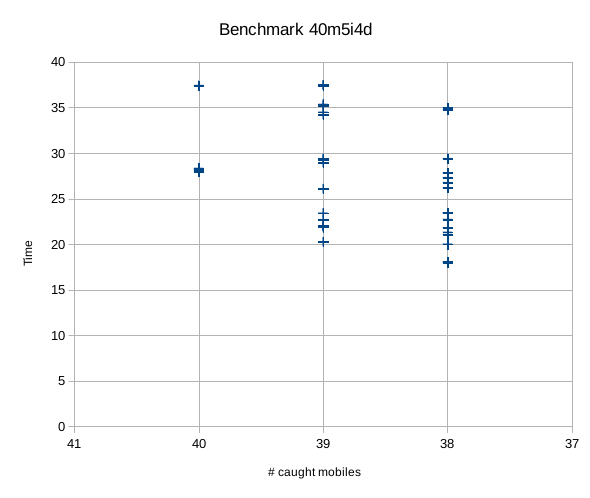
\includegraphics[width=.8\linewidth]{benchmark_40m5i4d}
		\caption{Positionnement des meilleures séquences (instance D)}
		\label{fig:best-seq-instanceD}
	\end{figure}


	\begin{table}[H]
		\centering
		\begin{tabular}{|l|l|l|}
		\hline
		Sequence             & Time    & Mobiles \\ \hline
		1 0 15 3 4 2 14 5    & 17.9825 & 38      \\ \hline
		3 1 14 4 5 10 0 15   & 17.9825 & 38      \\ \hline
		14 15 1 11 5 4 2 8   & 18.087  & 38      \\ \hline
		0 12 11 13 6 1 2 7   & 18.087  & 38      \\ \hline
		5 1 14 0 15 11 12 2  & 18.087  & 38      \\ \hline
		4 15 6 11 1 13 2 0   & 18.087  & 38      \\ \hline
		6 4 3 1 13 2 7 0     & 18.087  & 38      \\ \hline
		6 4 15 1 13 11 0 10  & 18.087  & 38      \\ \hline
		4 11 1 6 13 2 8 15   & 18.087  & 38      \\ \hline
		4 5 14 3 15 1 10 8   & 18.087  & 38      \\ \hline
		7 13 1 4 11 10 8 14  & 18.087  & 38      \\ \hline
		4 6 0 15 1 11 13 10  & 18.087  & 38      \\ \hline
		0 11 5 1 15 14 2 12  & 20.0344 & 38      \\ \hline
		15 11 1 8 2 4 14 5   & 20.0344 & 38      \\ \hline
		11 14 1 7 2 5 4 0    & 20.0344 & 38      \\ \hline
		6 15 11 12 8 5 1 2   & 20.2842 & 39      \\ \hline
		3 0 1 14 5 10 7 4    & 21.1011 & 38      \\ \hline
		1 11 2 13 15 4 0 6   & 21.3335 & 38      \\ \hline
		14 0 4 9 15 11 5 10  & 21.8098 & 38      \\ \hline
		3 0 2 7 5 12 9 14    & 21.8896 & 39      \\ \hline
		3 2 12 6 9 15 13 8   & 21.8896 & 39      \\ \hline
		3 5 2 14 1 4 7 0     & 21.9837 & 39      \\ \hline
		12 5 7 3 2 6 0 1     & 22.0176 & 39      \\ \hline
		14 12 3 15 0 13 10 1 & 22.0176 & 39      \\ \hline
		4 5 3 2 1 6 15 8     & 22.0176 & 39      \\ \hline
		13 11 7 14 12 1 8 2  & 22.0675 & 39      \\ \hline
		11 6 4 2 7 0 5 9     & 22.0675 & 39      \\ \hline
		3 0 4 13 6 2 9 15    & 22.728  & 39      \\ \hline
		6 3 0 12 13 15 9 10  & 22.7461 & 38      \\ \hline
		3 10 9 8 7 4 13 6    & 23.4357 & 39      \\ \hline
		3 6 9 7 10 12 13 0   & 23.4357 & 38      \\ \hline
		13 7 1 4 2 11 14 0   & 23.4669 & 38      \\ \hline
		0 6 11 5 4 1 10 15   & 26.11   & 39      \\ \hline
		15 1 2 14 5 8 11 12  & 26.2378 & 38      \\ \hline
		13 1 2 3 7 14 0 4    & 26.2378 & 38      \\ \hline
		11 7 1 12 13 0 10 14 & 26.7904 & 38      \\ \hline
		5 7 14 11 9 10 4 8   & 27.3375 & 38      \\ \hline
		12 1 7 10 13 14 11 0 & 27.8347 & 38      \\ \hline
		0 15 13 11 9 6 2 12  & 28.016  & 40      \\ \hline
		0 7 6 11 13 9 4 10   & 28.016  & 40      \\ \hline
		15 4 3 8 9 5 2 14    & 28.1546 & 40      \\ \hline
		13 12 8 1 7 6 2 11   & 28.2959 & 40      \\ \hline
		\end{tabular}
		\caption{Meilleures séquences pour l'instance D}
		\label{tab:best-seq-instanceD}
	\end{table}


	\section*{Instance E}


	\begin{table}[H]
		\centering
		\begin{tabular}{|l|l|l|}
		\hline
		Sequence             & Time    & Mobiles \\ \hline
		3 1 14 4 5 10 0 15   & 18.9738 & 60      \\ \hline
		9 14 3 12 2 7 0 13   & 18.9738 & 60      \\ \hline
		6 3 0 12 13 15 9 10  & 18.9738 & 60      \\ \hline
		3 0 4 13 6 2 9 15    & 18.9738 & 60      \\ \hline
		7 13 1 4 11 10 8 14  & 18.9738 & 60      \\ \hline
		12 5 7 3 2 6 0 1     & 19.1491 & 60      \\ \hline
		14 12 3 15 0 13 10 1 & 19.1491 & 60      \\ \hline
		15 4 3 8 9 5 2 14    & 19.1491 & 60      \\ \hline
		6 4 3 1 13 2 7 0     & 19.1491 & 60      \\ \hline
		4 5 3 2 1 6 15 8     & 19.1491 & 60      \\ \hline
		12 7 13 3 14 9 0 10  & 19.1491 & 60      \\ \hline
		8 4 9 5 15 14 3 10   & 19.1491 & 60      \\ \hline
		12 8 9 5 3 14 15 10  & 19.1491 & 60      \\ \hline
		4 5 14 3 15 1 10 8   & 19.1491 & 60      \\ \hline
		0 12 11 13 6 1 2 7   & 19.3372 & 60      \\ \hline
		1 0 15 3 4 2 14 5    & 19.3372 & 60      \\ \hline
		4 15 6 11 1 13 2 0   & 19.3372 & 60      \\ \hline
		4 11 1 6 13 2 8 15   & 19.3372 & 60      \\ \hline
		5 15 3 4 14 10 9 8   & 19.3372 & 60      \\ \hline
		0 6 11 5 4 1 10 15   & 19.3372 & 60      \\ \hline
		1 13 6 7 3 8 12 2    & 19.3372 & 60      \\ \hline
		0 7 6 11 13 9 4 10   & 19.3372 & 60      \\ \hline
		12 11 7 14 0 5 10 9  & 19.3946 & 60      \\ \hline
		14 0 4 9 15 11 5 10  & 19.3946 & 60      \\ \hline
		6 4 15 1 13 11 0 10  & 19.3946 & 60      \\ \hline
		4 6 0 15 1 11 13 10  & 19.3946 & 60      \\ \hline
		3 10 9 8 7 4 13 6    & 19.685  & 60      \\ \hline
		3 0 2 7 5 12 9 14    & 19.685  & 60      \\ \hline
		3 0 1 14 5 10 7 4    & 19.685  & 60      \\ \hline
		3 6 9 7 10 12 13 0   & 19.685  & 60      \\ \hline
		3 2 12 6 9 15 13 8   & 19.685  & 60      \\ \hline
		3 5 2 14 1 4 7 0     & 19.685  & 60      \\ \hline
		13 7 12 9 8 6 3 2    & 20.4026 & 60      \\ \hline
		13 7 1 4 2 11 14 0   & 20.6814 & 60      \\ \hline
		6 7 12 8 2 5 1 11    & 20.6814 & 60      \\ \hline
		7 10 13 6 12 9 0 3   & 20.6814 & 60      \\ \hline
		13 0 7 6 10 9 11 4   & 20.6814 & 60      \\ \hline
		13 7 10 1 11 6 0 4   & 20.6814 & 60      \\ \hline
		0 7 13 4 10 11 1 14  & 20.7688 & 60      \\ \hline
		9 13 0 7 4 14 10 3   & 20.7688 & 60      \\ \hline
		8 7 4 10 13 6 3 9    & 20.7688 & 60      \\ \hline
		0 15 13 11 9 6 2 12  & 20.9227 & 60      \\ \hline
		\end{tabular}
		\caption{Meilleures séquences pour l'instance E}
		\label{tab:best-seq-instanceE}
	\end{table}

	\begin{figure}[H]
		\centering
		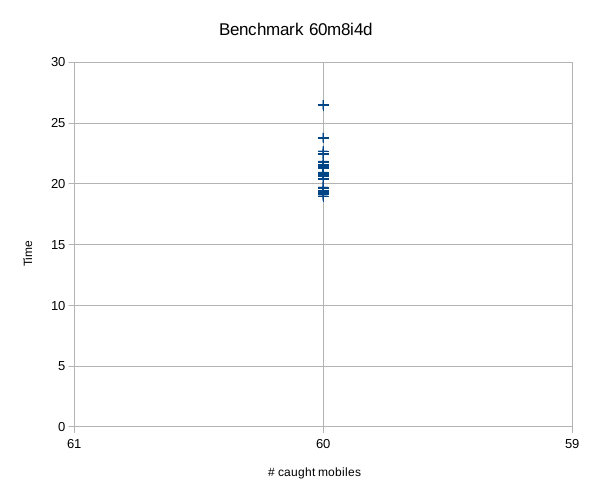
\includegraphics[width=.8\linewidth]{benchmark_60m8i4d}
		\caption{Positionnement des meilleures séquences (instance E)}
		\label{fig:best-seq-instanceE}
	\end{figure}


	\section*{Instance F}
	\begin{figure}[H]
		\centering
		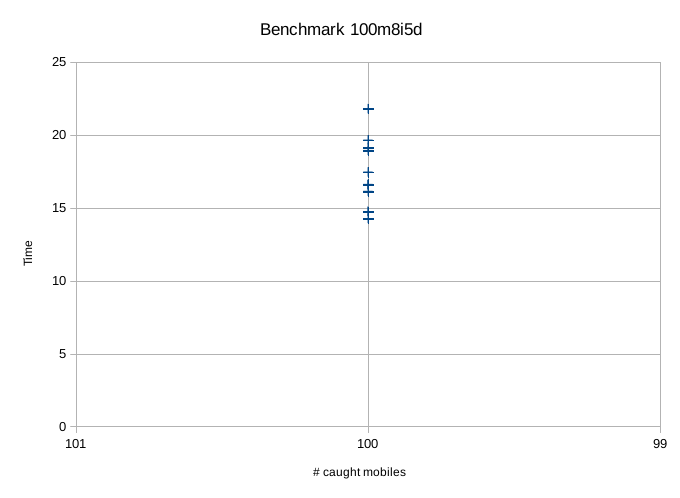
\includegraphics[width=.8\linewidth]{benchmark_100m8i5d}
		\caption{Positionnement des meilleures séquences (instance F)}
		\label{fig:best-seq-instanceF}
	\end{figure}

	\begin{table}[H]
		\centering
		\begin{tabular}{|l|l|l|}
		\hline
		Sequence             & Time    & Mobiles \\ \hline
		12 11 7 14 0 5 10 9  & 14.2699 & 100     \\ \hline
		14 12 3 15 0 13 10 1 & 14.2699 & 100     \\ \hline
		12 8 9 5 3 14 15 10  & 14.2699 & 100     \\ \hline
		4 5 14 3 15 1 10 8   & 14.2699 & 100     \\ \hline
		6 3 0 12 13 15 9 10  & 14.2699 & 100     \\ \hline
		4 8 15 13 2 9 6 11   & 14.7525 & 100     \\ \hline
		14 15 1 11 5 4 2 8   & 14.7525 & 100     \\ \hline
		5 0 12 14 15 9 2 11  & 14.7525 & 100     \\ \hline
		13 7 1 4 2 11 14 0   & 14.7525 & 100     \\ \hline
		1 0 15 3 4 2 14 5    & 14.7525 & 100     \\ \hline
		5 1 14 0 15 11 12 2  & 14.7525 & 100     \\ \hline
		6 7 12 8 2 5 1 11    & 14.7525 & 100     \\ \hline
		13 12 8 1 7 6 2 11   & 14.7525 & 100     \\ \hline
		12 5 7 3 2 6 0 1     & 14.7525 & 100     \\ \hline
		4 15 6 11 1 13 2 0   & 14.7525 & 100     \\ \hline
		14 0 4 9 15 11 5 10  & 14.7525 & 100     \\ \hline
		15 4 3 8 9 5 2 14    & 14.7525 & 100     \\ \hline
		11 7 1 12 13 0 10 14 & 14.7525 & 100     \\ \hline
		6 4 15 1 13 11 0 10  & 14.7525 & 100     \\ \hline
		6 15 11 12 8 5 1 2   & 14.7525 & 100     \\ \hline
		13 11 7 14 12 1 8 2  & 14.7525 & 100     \\ \hline
		12 7 13 3 14 9 0 10  & 14.7525 & 100     \\ \hline
		0 7 13 4 10 11 1 14  & 14.7525 & 100     \\ \hline
		5 15 3 4 14 10 9 8   & 14.7525 & 100     \\ \hline
		8 4 9 5 15 14 3 10   & 14.7525 & 100     \\ \hline
		9 13 0 7 4 14 10 3   & 14.7525 & 100     \\ \hline
		13 7 12 9 8 6 3 2    & 14.7525 & 100     \\ \hline
		1 13 6 7 3 8 12 2    & 14.7525 & 100     \\ \hline
		9 12 15 0 6 13 2 3   & 14.7525 & 100     \\ \hline
		8 7 4 10 13 6 3 9    & 14.7525 & 100     \\ \hline
		15 4 9 13 2 11 8 6   & 14.7525 & 100     \\ \hline
		7 13 1 4 11 10 8 14  & 14.7525 & 100     \\ \hline
		4 6 0 15 1 11 13 10  & 14.7525 & 100     \\ \hline
		12 1 7 10 13 14 11 0 & 14.7525 & 100     \\ \hline
		0 7 6 11 13 9 4 10   & 14.7525 & 100     \\ \hline
		13 11 1 4 14 8 10 7  & 16.1354 & 100     \\ \hline
		11 6 4 2 7 0 5 9     & 16.1354 & 100     \\ \hline
		0 6 11 5 4 1 10 15   & 16.1354 & 100     \\ \hline
		15 10 6 3 1 4 0 5    & 16.5785 & 100     \\ \hline
		5 7 14 11 9 10 4 8   & 16.5785 & 100     \\ \hline
		15 1 2 14 5 8 11 12  & 16.5785 & 100     \\ \hline
		0 15 13 11 9 6 2 12  & 16.5785 & 100     \\ \hline
		\end{tabular}
		\caption{Meilleures séquences pour l'instance F}
		\label{tab:best-seq-instanceF}
	\end{table}
